\documentclass{standalone}
\usepackage{tikz}
\usetikzlibrary{patterns, positioning}


\begin{document}
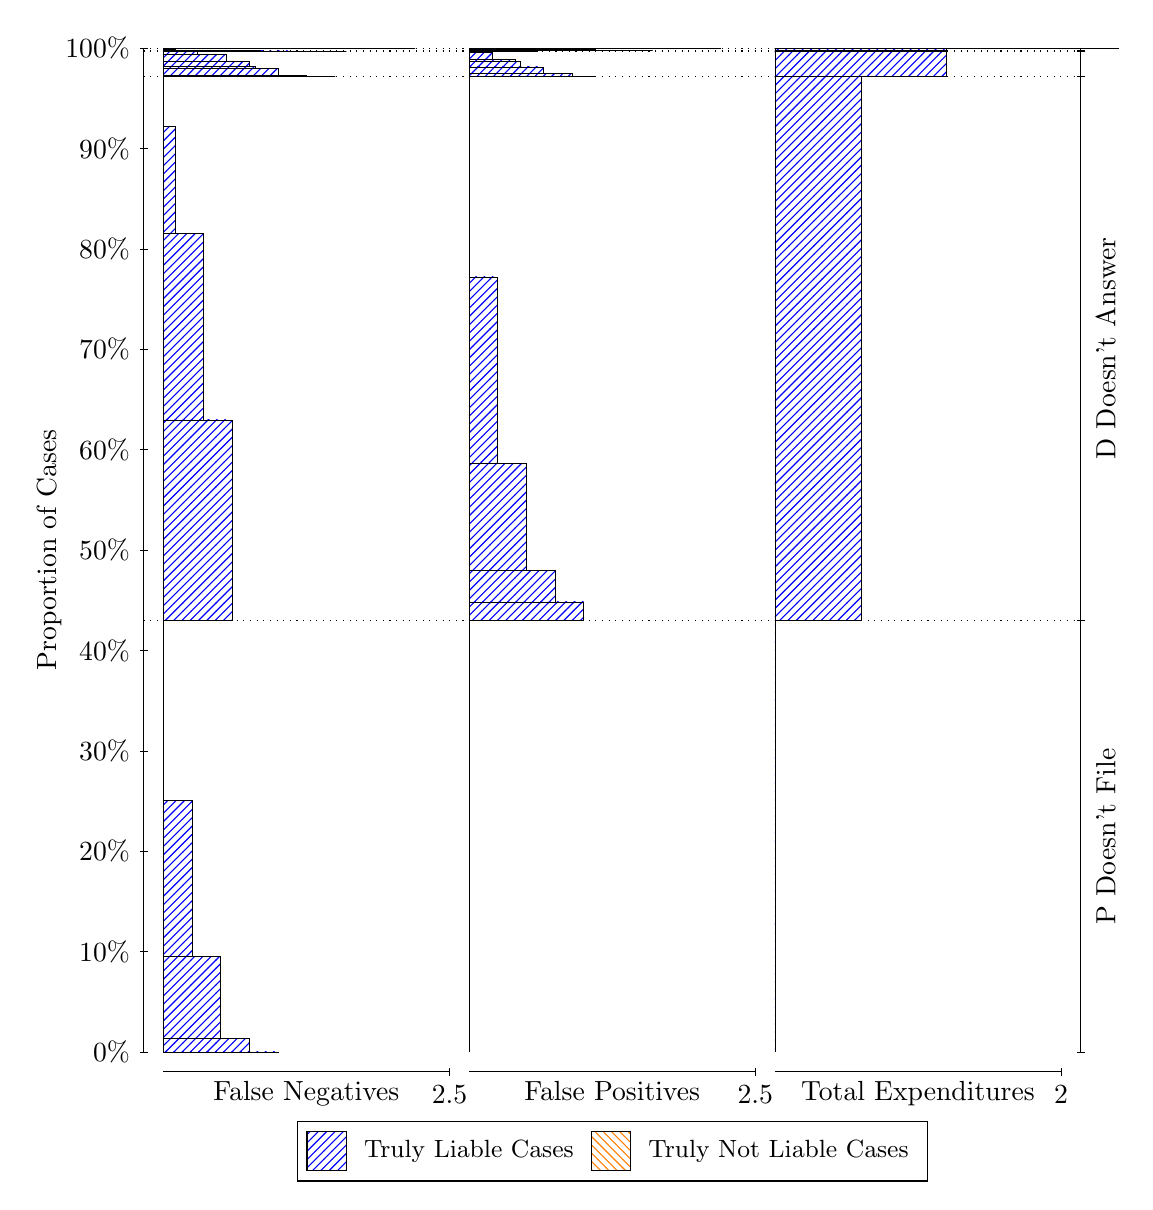
\begin{tikzpicture}
\draw[black, very thin] (1.5,1.75) -- (1.5,14.5);
\node[rotate=90, text=black, anchor=center] at (0.3, 8.125) {Proportion of Cases};
\draw[black, very thin] (1.45,1.75) -- (1.55,1.75);
\node[text=black, anchor=east] at (1.45, 1.75) {0\%};
\draw[black, very thin] (1.45,3.025) -- (1.55,3.025);
\node[text=black, anchor=east] at (1.45, 3.025) {10\%};
\draw[black, very thin] (1.45,4.3) -- (1.55,4.3);
\node[text=black, anchor=east] at (1.45, 4.3) {20\%};
\draw[black, very thin] (1.45,5.575) -- (1.55,5.575);
\node[text=black, anchor=east] at (1.45, 5.575) {30\%};
\draw[black, very thin] (1.45,6.85) -- (1.55,6.85);
\node[text=black, anchor=east] at (1.45, 6.85) {40\%};
\draw[black, very thin] (1.45,8.125) -- (1.55,8.125);
\node[text=black, anchor=east] at (1.45, 8.125) {50\%};
\draw[black, very thin] (1.45,9.4) -- (1.55,9.4);
\node[text=black, anchor=east] at (1.45, 9.4) {60\%};
\draw[black, very thin] (1.45,10.675) -- (1.55,10.675);
\node[text=black, anchor=east] at (1.45, 10.675) {70\%};
\draw[black, very thin] (1.45,11.95) -- (1.55,11.95);
\node[text=black, anchor=east] at (1.45, 11.95) {80\%};
\draw[black, very thin] (1.45,13.225) -- (1.55,13.225);
\node[text=black, anchor=east] at (1.45, 13.225) {90\%};
\draw[black, very thin] (1.45,14.5) -- (1.55,14.5);
\node[text=black, anchor=east] at (1.45, 14.5) {100\%};

\draw[black, very thin] (13.4,1.75) -- (13.4,14.5);
\draw[black, very thin] (13.35,1.75) -- (13.45,1.75);
\node[anchor=west] at (13.35, 1.75) {};
\draw[black, very thin] (13.35,7.2282) -- (13.45,7.2282);
\node[anchor=west] at (13.35, 7.2282) {};
\draw[black, very thin] (13.35,14.141) -- (13.45,14.141);
\node[anchor=west] at (13.35, 14.141) {};
\draw[black, very thin] (13.35,14.455) -- (13.45,14.455);
\node[anchor=west] at (13.35, 14.455) {};
\draw[black, very thin] (13.35,14.471) -- (13.45,14.471);
\node[anchor=west] at (13.35, 14.471) {};
\draw[black, very thin] (13.35,14.491) -- (13.45,14.491);
\node[anchor=west] at (13.35, 14.491) {};
\draw[black, very thin] (13.35,14.5) -- (13.45,14.5);
\node[anchor=west] at (13.35, 14.5) {};

\draw[black, very thin, pattern color=blue, pattern=north east lines] (1.75,1.75) rectangle (3.2033,1.7517);
\draw[black, very thin, pattern color=blue, pattern=north east lines] (1.75,1.7517) rectangle (2.84,1.9189);
\draw[black, very thin, pattern color=blue, pattern=north east lines] (1.75,1.9189) rectangle (2.4767,2.9681);
\draw[black, very thin, pattern color=blue, pattern=north east lines] (1.75,2.9681) rectangle (2.1133,4.9486);
\draw[black, very thin, pattern color=orange, pattern=north west lines] (1.75,4.9486) rectangle (1.75,4.9486);
\draw[black, very thin, pattern color=blue, pattern=north east lines] (1.75,4.9486) rectangle (1.75,7.2282);
\draw[black, very thin, pattern color=blue, pattern=north east lines] (1.75,7.2282) rectangle (2.622,9.7763);
\draw[black, very thin, pattern color=blue, pattern=north east lines] (1.75,9.7763) rectangle (2.2587,12.143);
\draw[black, very thin, pattern color=blue, pattern=north east lines] (1.75,12.143) rectangle (1.8953,13.5);
\draw[black, very thin, pattern color=orange, pattern=north west lines] (1.75,13.5) rectangle (1.75,13.5);
\draw[black, very thin, pattern color=blue, pattern=north east lines] (1.75,13.5) rectangle (1.75,14.141);
\draw[black, very thin, pattern color=blue, pattern=north east lines] (1.75,14.141) rectangle (3.93,14.141);
\draw[black, very thin, pattern color=blue, pattern=north east lines] (1.75,14.141) rectangle (3.7847,14.141);
\draw[black, very thin, pattern color=blue, pattern=north east lines] (1.75,14.141) rectangle (3.6393,14.141);
\draw[black, very thin, pattern color=blue, pattern=north east lines] (1.75,14.141) rectangle (3.5667,14.149);
\draw[black, very thin, pattern color=blue, pattern=north east lines] (1.75,14.149) rectangle (3.4213,14.15);
\draw[black, very thin, pattern color=blue, pattern=north east lines] (1.75,14.15) rectangle (3.3487,14.15);
\draw[black, very thin, pattern color=blue, pattern=north east lines] (1.75,14.15) rectangle (3.276,14.151);
\draw[black, very thin, pattern color=blue, pattern=north east lines] (1.75,14.151) rectangle (3.2033,14.238);
\draw[black, very thin, pattern color=blue, pattern=north east lines] (1.75,14.238) rectangle (3.058,14.239);
\draw[black, very thin, pattern color=blue, pattern=north east lines] (1.75,14.239) rectangle (2.9853,14.24);
\draw[black, very thin, pattern color=blue, pattern=north east lines] (1.75,14.24) rectangle (2.9127,14.264);
\draw[black, very thin, pattern color=blue, pattern=north east lines] (1.75,14.264) rectangle (2.84,14.335);
\draw[black, very thin, pattern color=blue, pattern=north east lines] (1.75,14.335) rectangle (2.6947,14.335);
\draw[black, very thin, pattern color=blue, pattern=north east lines] (1.75,14.335) rectangle (2.622,14.335);
\draw[black, very thin, pattern color=blue, pattern=north east lines] (1.75,14.335) rectangle (2.5493,14.422);
\draw[black, very thin, pattern color=blue, pattern=north east lines] (1.75,14.422) rectangle (2.4767,14.423);
\draw[black, very thin, pattern color=blue, pattern=north east lines] (1.75,14.423) rectangle (2.3313,14.423);
\draw[black, very thin, pattern color=blue, pattern=north east lines] (1.75,14.423) rectangle (2.2587,14.423);
\draw[black, very thin, pattern color=blue, pattern=north east lines] (1.75,14.423) rectangle (2.186,14.455);
\draw[black, very thin, pattern color=blue, pattern=north east lines] (1.75,14.455) rectangle (1.8953,14.455);
\draw[black, very thin, pattern color=orange, pattern=north west lines] (1.75,14.455) rectangle (1.75,14.455);
\draw[black, very thin, pattern color=blue, pattern=north east lines] (1.75,14.455) rectangle (4.0753,14.455);
\draw[black, very thin, pattern color=blue, pattern=north east lines] (1.75,14.455) rectangle (3.712,14.456);
\draw[black, very thin, pattern color=blue, pattern=north east lines] (1.75,14.456) rectangle (3.3487,14.465);
\draw[black, very thin, pattern color=blue, pattern=north east lines] (1.75,14.465) rectangle (2.9853,14.471);
\draw[black, very thin, pattern color=blue, pattern=north east lines] (1.75,14.471) rectangle (2.622,14.471);
\draw[black, very thin, pattern color=orange, pattern=north west lines] (1.75,14.471) rectangle (1.75,14.471);
\draw[black, very thin, pattern color=blue, pattern=north east lines] (1.75,14.471) rectangle (2.622,14.471);
\draw[black, very thin, pattern color=blue, pattern=north east lines] (1.75,14.471) rectangle (2.2587,14.474);
\draw[black, very thin, pattern color=blue, pattern=north east lines] (1.75,14.474) rectangle (1.8953,14.489);
\draw[black, very thin, pattern color=orange, pattern=north west lines] (1.75,14.489) rectangle (1.75,14.489);
\draw[black, very thin, pattern color=blue, pattern=north east lines] (1.75,14.489) rectangle (1.75,14.491);
\draw[black, very thin, pattern color=blue, pattern=north east lines] (1.75,14.491) rectangle (4.9473,14.491);
\draw[black, very thin, pattern color=blue, pattern=north east lines] (1.75,14.491) rectangle (4.584,14.491);
\draw[black, very thin, pattern color=blue, pattern=north east lines] (1.75,14.491) rectangle (4.2207,14.491);
\draw[black, very thin, pattern color=blue, pattern=north east lines] (1.75,14.491) rectangle (3.8573,14.493);
\draw[black, very thin, pattern color=blue, pattern=north east lines] (1.75,14.493) rectangle (3.494,14.498);
\draw[black, very thin, pattern color=blue, pattern=north east lines] (1.75,14.498) rectangle (3.1307,14.5);
\draw[black, very thin, pattern color=blue, pattern=north east lines] (1.75,14.5) rectangle (2.7673,14.5);
\draw[black, very thin, pattern color=blue, pattern=north east lines] (1.75,14.5) rectangle (2.404,14.5);
\draw[black, very thin, pattern color=blue, pattern=north east lines] (1.75,14.5) rectangle (2.0407,14.5);
\draw[black, very thin, pattern color=orange, pattern=north west lines] (1.75,14.5) rectangle (1.75,14.5);
\draw[black, very thin, pattern color=orange, pattern=north west lines] (5.6333,1.75) rectangle (5.6333,1.75);
\draw[black, very thin, pattern color=blue, pattern=north east lines] (5.6333,1.75) rectangle (5.6333,7.2282);
\draw[black, very thin, pattern color=orange, pattern=north west lines] (5.6333,7.2282) rectangle (7.0867,7.2282);
\draw[black, very thin, pattern color=blue, pattern=north east lines] (5.6333,7.2282) rectangle (7.0867,7.4651);
\draw[black, very thin, pattern color=blue, pattern=north east lines] (5.6333,7.4651) rectangle (6.7233,7.8689);
\draw[black, very thin, pattern color=blue, pattern=north east lines] (5.6333,7.8689) rectangle (6.36,9.2258);
\draw[black, very thin, pattern color=blue, pattern=north east lines] (5.6333,9.2258) rectangle (5.9967,11.593);
\draw[black, very thin, pattern color=blue, pattern=north east lines] (5.6333,11.593) rectangle (5.6333,14.141);
\draw[black, very thin, pattern color=orange, pattern=north west lines] (5.6333,14.141) rectangle (7.232,14.141);
\draw[black, very thin, pattern color=blue, pattern=north east lines] (5.6333,14.141) rectangle (7.232,14.141);
\draw[black, very thin, pattern color=orange, pattern=north west lines] (5.6333,14.141) rectangle (6.9413,14.141);
\draw[black, very thin, pattern color=blue, pattern=north east lines] (5.6333,14.141) rectangle (6.9413,14.173);
\draw[black, very thin, pattern color=blue, pattern=north east lines] (5.6333,14.173) rectangle (6.8687,14.173);
\draw[black, very thin, pattern color=orange, pattern=north west lines] (5.6333,14.173) rectangle (6.796,14.173);
\draw[black, very thin, pattern color=blue, pattern=north east lines] (5.6333,14.173) rectangle (6.796,14.173);
\draw[black, very thin, pattern color=orange, pattern=north west lines] (5.6333,14.173) rectangle (6.6507,14.173);
\draw[black, very thin, pattern color=blue, pattern=north east lines] (5.6333,14.173) rectangle (6.6507,14.174);
\draw[black, very thin, pattern color=blue, pattern=north east lines] (5.6333,14.174) rectangle (6.578,14.26);
\draw[black, very thin, pattern color=blue, pattern=north east lines] (5.6333,14.26) rectangle (6.5053,14.261);
\draw[black, very thin, pattern color=blue, pattern=north east lines] (5.6333,14.261) rectangle (6.4327,14.261);
\draw[black, very thin, pattern color=blue, pattern=north east lines] (5.6333,14.261) rectangle (6.2873,14.331);
\draw[black, very thin, pattern color=blue, pattern=north east lines] (5.6333,14.331) rectangle (6.2147,14.356);
\draw[black, very thin, pattern color=blue, pattern=north east lines] (5.6333,14.356) rectangle (6.142,14.357);
\draw[black, very thin, pattern color=blue, pattern=north east lines] (5.6333,14.357) rectangle (6.0693,14.358);
\draw[black, very thin, pattern color=blue, pattern=north east lines] (5.6333,14.358) rectangle (5.924,14.445);
\draw[black, very thin, pattern color=blue, pattern=north east lines] (5.6333,14.445) rectangle (5.8513,14.446);
\draw[black, very thin, pattern color=blue, pattern=north east lines] (5.6333,14.446) rectangle (5.7787,14.446);
\draw[black, very thin, pattern color=blue, pattern=north east lines] (5.6333,14.446) rectangle (5.706,14.447);
\draw[black, very thin, pattern color=blue, pattern=north east lines] (5.6333,14.447) rectangle (5.6333,14.455);
\draw[black, very thin, pattern color=orange, pattern=north west lines] (5.6333,14.455) rectangle (6.5053,14.455);
\draw[black, very thin, pattern color=blue, pattern=north east lines] (5.6333,14.455) rectangle (6.5053,14.455);
\draw[black, very thin, pattern color=blue, pattern=north east lines] (5.6333,14.455) rectangle (6.142,14.462);
\draw[black, very thin, pattern color=blue, pattern=north east lines] (5.6333,14.462) rectangle (5.7787,14.47);
\draw[black, very thin, pattern color=blue, pattern=north east lines] (5.6333,14.47) rectangle (5.6333,14.471);
\draw[black, very thin, pattern color=orange, pattern=north west lines] (5.6333,14.471) rectangle (7.9587,14.471);
\draw[black, very thin, pattern color=blue, pattern=north east lines] (5.6333,14.471) rectangle (7.9587,14.471);
\draw[black, very thin, pattern color=blue, pattern=north east lines] (5.6333,14.471) rectangle (7.5953,14.473);
\draw[black, very thin, pattern color=blue, pattern=north east lines] (5.6333,14.473) rectangle (7.232,14.487);
\draw[black, very thin, pattern color=blue, pattern=north east lines] (5.6333,14.487) rectangle (6.8687,14.491);
\draw[black, very thin, pattern color=blue, pattern=north east lines] (5.6333,14.491) rectangle (6.5053,14.491);
\draw[black, very thin, pattern color=orange, pattern=north west lines] (5.6333,14.491) rectangle (8.8307,14.491);
\draw[black, very thin, pattern color=blue, pattern=north east lines] (5.6333,14.491) rectangle (8.8307,14.491);
\draw[black, very thin, pattern color=blue, pattern=north east lines] (5.6333,14.491) rectangle (8.4673,14.491);
\draw[black, very thin, pattern color=orange, pattern=north west lines] (5.6333,14.491) rectangle (8.4673,14.491);
\draw[black, very thin, pattern color=blue, pattern=north east lines] (5.6333,14.491) rectangle (8.4673,14.491);
\draw[black, very thin, pattern color=blue, pattern=north east lines] (5.6333,14.491) rectangle (8.104,14.491);
\draw[black, very thin, pattern color=orange, pattern=north west lines] (5.6333,14.491) rectangle (8.104,14.491);
\draw[black, very thin, pattern color=blue, pattern=north east lines] (5.6333,14.491) rectangle (8.104,14.491);
\draw[black, very thin, pattern color=blue, pattern=north east lines] (5.6333,14.491) rectangle (7.7407,14.491);
\draw[black, very thin, pattern color=orange, pattern=north west lines] (5.6333,14.491) rectangle (7.7407,14.491);
\draw[black, very thin, pattern color=blue, pattern=north east lines] (5.6333,14.491) rectangle (7.7407,14.493);
\draw[black, very thin, pattern color=blue, pattern=north east lines] (5.6333,14.493) rectangle (7.3773,14.493);
\draw[black, very thin, pattern color=orange, pattern=north west lines] (5.6333,14.493) rectangle (7.3773,14.493);
\draw[black, very thin, pattern color=blue, pattern=north east lines] (5.6333,14.493) rectangle (7.3773,14.498);
\draw[black, very thin, pattern color=blue, pattern=north east lines] (5.6333,14.498) rectangle (7.014,14.5);
\draw[black, very thin, pattern color=blue, pattern=north east lines] (5.6333,14.5) rectangle (6.6507,14.5);
\draw[black, very thin, pattern color=blue, pattern=north east lines] (5.6333,14.5) rectangle (6.2873,14.5);
\draw[black, very thin, pattern color=blue, pattern=north east lines] (5.6333,14.5) rectangle (5.924,14.5);
\draw[black, very thin, pattern color=orange, pattern=north west lines] (9.5167,1.75) rectangle (9.5167,1.75);
\draw[black, very thin, pattern color=blue, pattern=north east lines] (9.5167,1.75) rectangle (9.5167,7.2282);
\draw[black, very thin, pattern color=orange, pattern=north west lines] (9.5167,7.2282) rectangle (10.607,7.2282);
\draw[black, very thin, pattern color=blue, pattern=north east lines] (9.5167,7.2282) rectangle (10.607,14.141);
\draw[black, very thin, pattern color=orange, pattern=north west lines] (9.5167,14.141) rectangle (11.697,14.141);
\draw[black, very thin, pattern color=blue, pattern=north east lines] (9.5167,14.141) rectangle (11.697,14.142);
\draw[black, very thin, pattern color=orange, pattern=north west lines] (9.5167,14.142) rectangle (11.697,14.142);
\draw[black, very thin, pattern color=blue, pattern=north east lines] (9.5167,14.142) rectangle (11.697,14.455);
\draw[black, very thin, pattern color=orange, pattern=north west lines] (9.5167,14.455) rectangle (11.697,14.455);
\draw[black, very thin, pattern color=blue, pattern=north east lines] (9.5167,14.455) rectangle (11.697,14.471);
\draw[black, very thin, pattern color=orange, pattern=north west lines] (9.5167,14.471) rectangle (11.697,14.471);
\draw[black, very thin, pattern color=blue, pattern=north east lines] (9.5167,14.471) rectangle (11.697,14.491);
\draw[black, very thin, pattern color=orange, pattern=north west lines] (9.5167,14.491) rectangle (13.877,14.491);
\draw[black, very thin, pattern color=blue, pattern=north east lines] (9.5167,14.491) rectangle (13.877,14.491);
\draw[black, very thin, pattern color=orange, pattern=north west lines] (9.5167,14.491) rectangle (13.877,14.491);
\draw[black, very thin, pattern color=blue, pattern=north east lines] (9.5167,14.491) rectangle (13.877,14.5);
\draw[black, dotted] (1.5,7.2282) -- (13.4,7.2282);
\draw[black, dotted] (1.5,14.141) -- (13.4,14.141);
\draw[black, dotted] (1.5,14.455) -- (13.4,14.455);
\draw[black, dotted] (1.5,14.471) -- (13.4,14.471);
\draw[black, dotted] (1.5,14.491) -- (13.4,14.491);
\draw[black, very thin] (1.75,1.5) -- (5.3833,1.5);
\node[text=black, anchor=north] at (3.5667, 1.5) {False Negatives};
\draw[black, very thin] (5.3833,1.45) -- (5.3833,1.55);
\node[text=black, anchor=north] at (5.3833, 1.45) {2.5};

\draw[black, very thin] (5.6333,1.5) -- (9.2667,1.5);
\node[text=black, anchor=north] at (7.45, 1.5) {False Positives};
\draw[black, very thin] (9.2667,1.45) -- (9.2667,1.55);
\node[text=black, anchor=north] at (9.2667, 1.45) {2.5};

\draw[black, very thin] (9.5167,1.5) -- (13.15,1.5);
\node[text=black, anchor=north] at (11.333, 1.5) {Total Expenditures};
\draw[black, very thin] (13.15,1.45) -- (13.15,1.55);
\node[text=black, anchor=north] at (13.15, 1.45) {2};

\node[text=black, centered, rotate=90] at (13.72, 4.4891) {P Doesn't File};
\node[text=black, centered, rotate=90] at (13.72, 10.684) {D Doesn't Answer};





\draw (7.449999999999999,1.5) node[draw=none] (baseCoordinate) {};
\begin{scope}[align=center]
        \matrix[scale=0.5, draw=black, below=0.5cm of baseCoordinate, nodes={draw}, column sep=0.1cm]{
            \node[rectangle, draw, minimum width=0.5cm, minimum height=0.5cm, pattern color=blue, pattern=north east lines] {}; &
            \node[draw=none, font=\small, text=black] (B) {Truly Liable Cases}; &
            \node[rectangle, draw, minimum width=0.5cm, minimum height=0.5cm, pattern color=orange, pattern=north west lines] {}; &
            \node[draw=none, font=\small, text=black] (B) {Truly Not Liable Cases}; \\
            };
\end{scope}

\end{tikzpicture}
\end{document}